%\subsubsection{TOTUS data store setup}
%Figure \ref{fig:totus_setup_flow} shows the workflow to setup the data store for TOTUS.
%\begin{landscape}
%	\begin{figure}[h]
%		 \caption{TOTUS setup workflow}
%		 \label{fig:totus_setup_flow}
%		 \missingfigure{Workflow diagram for TOTUS setup and data loading}
%		  %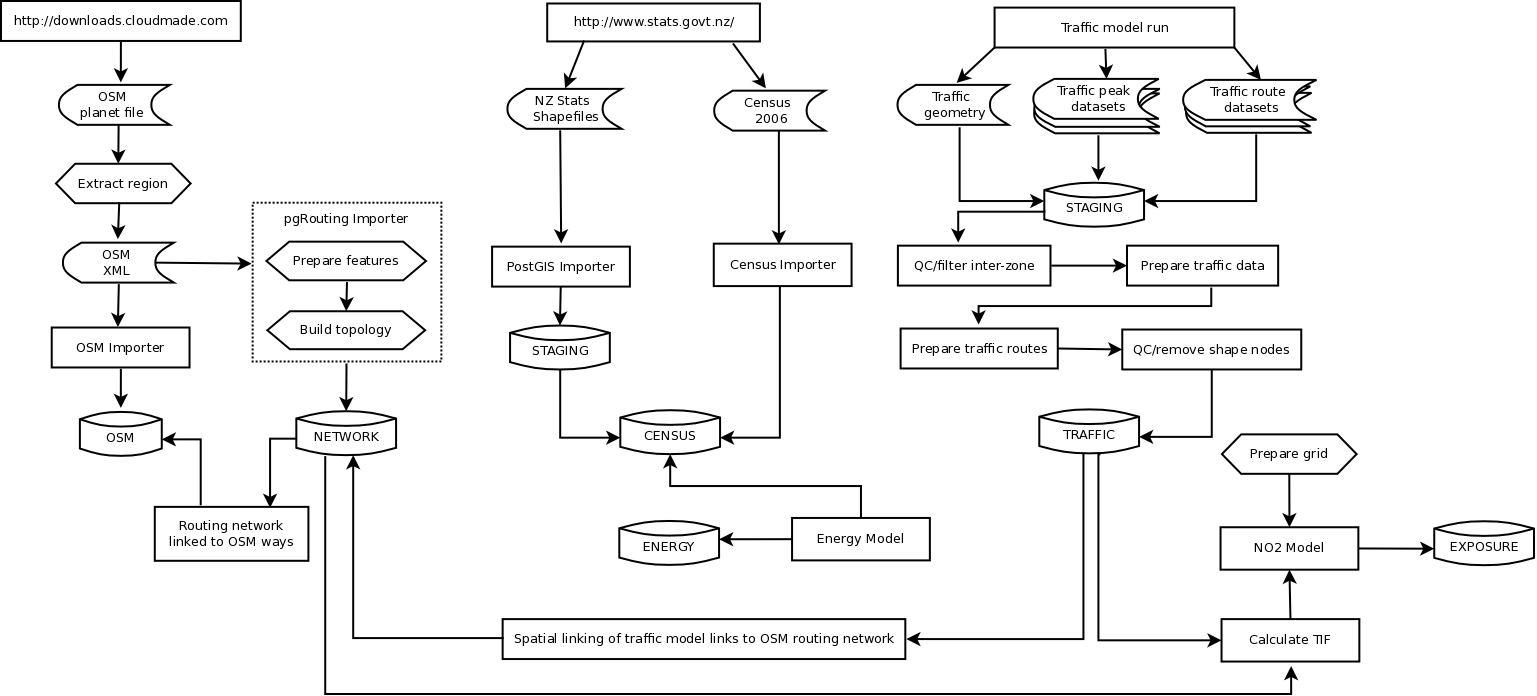
\includegraphics[width=\linewidth]{./system_preparation.png}
%		   % system_preparation.png: 1537x696 pixel, 51dpi, 76.85x34.80 cm, bb=0 0 2178 986
%	\end{figure}
%\end{landscape}

TOTUS is a very flexible system that can be configured to use several different data layers but the minimum expected are:
\begin{itemize}
	\item \textbf{Traffic network}. The road network is defined using data from the Open Street Map (OSM) project\cite{dummy_temp}\todo{Add reference to OSM project}.
	\item \textbf{Traffic data}. As a long term planning and assessment tool, TOTUS expects data from a strategic traffic model for information about the traffic flows on the network and the fleet composition.
	\item \textbf{Demographic data}. The third data source is the census information that should cover the same geographical area as the traffic network data.
\end{itemize}

